\documentclass[tikz]{standalone}
\usepackage{amsmath}
\usepackage{amssymb}
\usepackage{amsfonts}
\usepackage{tikz}
\usetikzlibrary{calc}

\thispagestyle{empty}
\begin{document}
 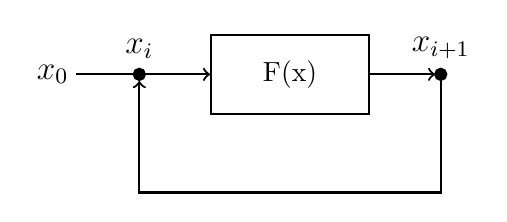
\begin{tikzpicture}[thick]

% Rectangle with F(x)
\node[draw, rectangle, minimum width=2cm, minimum height=1cm] (block) at (0,0) {F(x)};

% Input arrow with circle node
\coordinate (instart) at ($(block.west)+(-1.7,0)$);
\coordinate (inmid) at ($(block.west)+(-0.9,0)$);
\draw[->] (instart) -- (block.west);
\node[draw, circle, minimum size=4pt, inner sep=0pt, fill=black] (leftnode) at (inmid) {};

% Output arrow with circle node
\coordinate (outmid) at ($(block.east)+(0.9,0)$);
\draw[->] (block.east) -- ($(outmid.west)-(0.07,0)$);
\node[draw, circle, minimum size=4pt, inner sep=0pt, fill=black] (rightnode) at (outmid) {};

% Labels
\node at ($(instart)+(-0.3,0)$) {\large $x_{0}$};
%\node at ($(outend)+(0.5,0)$) {\large $x_{i+1}$};

\node[above=2pt] at (leftnode) {\large $x_i$};
\node[above=2pt] at (rightnode) {\large $x_{i+1}$};

% Feedback arrow from right circle to left circle
\coordinate (fbdown) at ($(rightnode)+(0,-1.5)$);
\coordinate (fbleft) at ($(leftnode)+(0,-1.5)$);
\draw[->] (rightnode) -- (fbdown) -- (fbleft) -- (leftnode);
\end{tikzpicture}

\end{document}
